% This file is part of the Apogee project.
% Copyright 2014 Melissa Ness and David W. Hogg.

% # short-term to-do
% - draft abstract
% - draft introduction

% # style notes
% - are they ``labels'' or ``labels''?  MKN:  Make a call and audit the whole text.
% - needs a name and to use it consistently as \thename

\documentclass[12pt, preprint]{aastex}
\usepackage{bm}
\input{vc}
\newcommand{\sectionname}{Section}
\newcommand{\documentname}{\textsl{Note}}


\usepackage{graphicx}
\usepackage{subfigure}
\usepackage{amsmath}

\newcommand{\set}[1]{\bm{#1}}
\newcommand{\mean}[1]{\overline{#1}}
\newcommand{\given}{\,|\,}
\newcommand{\teff}{\mbox{$\rm T_{eff}$}}
\newcommand{\kms}{\mbox{$\rm ks^{-1} k$}}
\newcommand{\feh}{\mbox{$\rm [Fe/H]$}}
\newcommand{\logg}{\mbox{$\rm \log g$}}
%\newcommand{\tc}{\fontfamily{qcr}\selectfont}
\newcommand{\tc}{\textsl{The Cannon}} 
\newcommand{\apogee}{\textsl{APOGEE}} 
\newcommand{\apokasc}{\textsl{APOKASC}} 
\newcommand{\galah}{\textsl{GALAH}} 
\newcommand{\aspcap}{\textsl{ASPCAP}} 
\newcommand{\gaiaeso}{\textsl{Gaia-ESO}} 
\newcommand{\gaia}{\textsl{GAIA}} 
\newcommand{\matisse}{\textsl{Matisse}} 


 


\usepackage{morefloats}

\begin{document}

\title{\textsc{\tc:} Wavelength-independent stellar parameter determination using data-driven models}
\author{
  MKN,
  DWH,
  \&
  HWR,
  GZ, AH} 
\date{DRAFT / \gitdate\ / \githash\ / NOT FOR DISTRIBUTION}

% DWH say: Obey A&A abstract rules (ish).
%          They offer good guidance on abstract construction.
% read/ref that paper DWH sent through
% reference matisse somewhere. 


\begin{abstract}

Context: There are now numerous large programs to survey stars in the Milky Way, each of which is investing significant effort to determine and deliver stellar parameters and individual abundances across different wavelength regions. We present a generalised and wavelength independent regression technique to determine stellar parameters for large surveys, using a model built from data. Our approach does not require an intricate line-list characterisation at each new wavelength region observed by a survey, nor is it penalised by uncertainties in stellar models across different bands. With this methodology we effectively characterise how each pixel in a spectrum contributes to a given stellar parameter or label used to describe a star. In exploiting every pixel, we can determine stellar parameters at a fraction of the signal to noise compared to other techniques, for a given uncertainty. \\
Aims: We present \tc, our regression analysis approach which returns labels for stars from large datasets, using data-driven models.  Our method transfers labels (of \teff, \logg\ and [Fe/H]) from a training set of data whose parameters are well determined (i.e. members of open and globular clusters) to the entire set of stars in a survey. Our work motivates the importance of having an established set of standard stars with well-determined labels. Given such standard calibrators, it is possible, via this technique of label-transfer, to place every stellar survey of the Milky Way on the same stellar parameter scale and homogeneously map the stellar population of the Milky Way from Northern and Southern hemispheres and using different wavelength regions. \\
Methods: We demonstrate \tc\ using the \apogee\ dataset, to transfer labels from a training set of data comprising 550 stars from 19 open and globular clusters observed in \textit{APOGEE}, to every new star observed in the \apogee\ DR10 data release. \\
Results:   Using only 550 training stars with \textit{known} labels to construct our model, we reproduce the stellar parameters for the stars in the \apogee\ survey from DR10, to \teff\ --12 $\pm$ 87 K, \logg\ --0.04 $\pm$ 0.18 and \feh\ +0.01 $\pm$ 0.08. The rms error between our results and that of \apogee\ is comparable to the error estimates in each of their parameters. As our approach has extremely small intrinsic errors,  we can determine the stellar parameters at a fraction (25\%) of the signal to noise required by minimisation techniques. Our method is expandable to additional labels and relevant for chemical tagging and motivates the importance of having a ``gold standard'' set of stars studied at high resolution. 



\end{abstract}

\section{Introduction}

There are numerous challenges in exploiting the large datasets of stellar spectra that have become available only in recent years. The first of these is the determination of stellar parameters which is typically a significant and iterative effort, customised specifically to the particular wavelength region of a given survey. Furthermore, different methods and groups obtain different results for the same stars, even within the same survey due to different input assumptions and methods. For example, despite adopting the same line list and stellar models, the 13 GES nodes which provide abundance measurements for the GES data via different methodologies, obtain different stellar parameter measurements  \citep{Smiljanic2014}, which are subsequently combined as a way of homogenising the data.  Stellar models are almost always explicitly relied upon for stellar parameter determination, which are incomplete and simplified e.g. 1D models are adopted, which  largely do not account for different molecular opacities, convection, dust, non linear thermal equilibrium effects, stellar winds and the stellar chromosphere. Typically, to determine stellar parameters, stellar models are used to derive a best-fit spectrum using some minimisation technique across an often masked portion of the spectrum, determined from linelists to be most reliable or relevant and a post-calibration procedure is then applied, using for example benchmark stars studied at high resolution or well characterised open and globular cluster stars. The inputs to these procedures, uncertainties and assumptions vary between surveys so different surveys are on different stellar parameter scales; this belies a second major challenge of the era of large datasets. 

An optimal exploitation of all of the datasets present and future including \apogee\, \gaiaeso, \galah\ and \gaia\ relies on their homogenisation, i.e. a consistent stellar parameter scale for stars that have been observed by the Northern and Southern surveys, which operate across different wavelength regions. To facilitate this effort there is typically some calibration stars in common observed between surveys. These may be stars studied and characterised at high resolution in the optical wavelength region and also globular and open clusters which have well determined labels. Rather than simply being used to post-calibrate surveys to a standardised physical scale, these calibration or standard stars afford a critical opportunity to create a data-driven model.  This data-driven model can be used for label-transfer (e.g. for labels of stellar parameters and individual abundances) from the calibration set to new stars in the survey. This relies on the parameter range and quality of the calibration set of stars and that they are observed between the different surveys and have a consistently defined and adopted set of labels. 

In addition to the challenges, there are numerous opportunities in this era of large surveys of the Milky Way to characterise the information in the data itself, by building data-driven models and implementing a differential analysis on large datasets. This can not only circumvent issues with using flawed stellar models to determine stellar parameters and detailed abundances, but also identify where and how models diverge from data. We use the \apogee\ dataset to demonstrate the power of and information content in the data itself to implement a regression technique using a data-driven model to determine stellar parameter determination via label-transfer. Our aim is distinct from simply determining parameters and we seek not to find the best fit spectra similarly to minimisation techniques. Our aim is to implement a procedure which makes it possible to understand and characterise the spectra as a function of the labels which describe it. 

Although we present the methodology of using label-transfer to efficiently and effectively determine stellar parameters for a large survey using the example of the \apogee\ survey, this method can be used for \textit{all} stellar surveys, directly.  Our methodology is very relevant for chemical tagging in large datasets, as it can formally describe and differentiate the spectra in multiple-abundance space, given an extension of the input labels.  Our basic implementation of \tc\ that we present implements only three labels, but this can easily be extended to additional labels  (e.g. [$\alpha$/Fe], [X/Fe], age) and also more comprehensive models (e.g. Gaussian processes) , which we describe in detail in the Discussion. Additionally, as we are using the information in every pixel, this methodology should perform at lower signal to noise than minimisation techniques and provide a quantification of data driven spectra comparison and differentiation, which may be a key tool in exploring the archeology of stars via chemical tagging. 

Our overarching aim of describing stellar flux as a function of stellar labels is not dissimilar from the MATrix Inversion for Spectral SythEsis (\matisse) procedure for derivation of stellar parameters \citep{Reico-Blanco2006}, but \matisse\ employs a large grid of synthetic spectra and characterises a set of basis vectors which project onto each observed spectrum to determine stellar labels by calculating an optimal combined synthetic spectrum describing the stellar flux. Conversely, we use a data-driven model and do not project onto any optimal combined theoretical spectrum. Rather we directly determine labels using a total of around 22,000 degrees of freedom of information in the data, given the 7200 pixels comprising flux and the 3 input labels that we return. % reword the above

We have adopted a bottom-up approach for this project, starting with the most basic implementation and upgrading this iteratively.  In laying out the methodology of this approach we firstly describe the \apogee\ dataset and the way we process the data for both training and test data. We then describe perhaps the simplest implementation of label-transfer possible, using a first-order linear model. This first-order model is insufficiently flexible to describe the labels of the stars and so we extended our model to quadratic form, which satisfactorily describes the parameter space of the training data. The success of this model is demonstrated by running \tc\ through the DR10 data available through the sdss-3 data server, the results for which we provide in an online machine-readable table. This simple model which we use to describe the label-transfer procedure implemented with  \tc\, demonstrates that this is an efficient, powerful and robust method that can be applied to all surveys. We discuss in detail how this first approach can be expanded to a more general form with additional labels, moving to a more comprehensive model that is likely necessary over a wider parameter range of stars. 

\textbf{- DWH: difference between what we are doing and what machine learning would do - i.e. given our methodology we can learn from the data. }


\section{Data}

The data we employ can be from any large survey. Here we use the \apogee\ data to showcase the label-transfer method of \tc\ . We describe how we process the input data to the program that is provided by APOGEE and similarly prepare the training data for the label transfer. 

\subsection{\apogee\ Data}

A robust flux normalisation of the spectra is critical and the flux normalisation must provide consistently scaled spectra across the range of stellar parameters and at different signal to noise ratios. We implement a continuum normalisation that is informed by our model by selecting continuum pixels as described in Section \ref{sec:results}, having first trained our model using \apogee\ training spectra that has been continuum normalised using a polynomial fit to a an upper quantile of the spectra in the APOGEE pipeline \citep{Meszaros2013}. 

The continuum normalisation we implement can be applied to either the \apogee\ pseudo-normalised spectra in the \textit{aspcapStar} fits files, which we adopt for our primary training and test data, or the \textit{apStar} full spectrum flux files provided as part of the DR10 data release. We use the \textit{apStar} files, which are reduced, resampled but not pre-continuum normalised, in order to evaluate the performance of \tc\ at lower signal to noise, by testing using the individual visit spectra provided in these files.  

The selected continuum pixels are used to fit a 3rd-order Chebyshev polynomial, treating each of the three chips separately and the contribution to the fit of each pixel is weighted by the inverse variance from the error array provided for each star in the \apogee\ fits files. Figure \ref{fig:norm} shows an example of this normalisation applied to spectra with different labels from \tc\, including stars at the high and low end of metallicity, temperature and gravity across the stellar parameter range of the data. The continuum pixels used for the Chebyshev polynomial fit are shown in the black points. These figures showcase the full spectral range of \apogee\ data. For a clearer impression of the spectral flux variation we use narrower regions marked in this Figure, (a) and (b), for all subsequent illustrations of the spectral data. 

%made with makecontin_data2.py
\begin{figure}[h!]
  \includegraphics[width=\hsize]{./plots/four_examples2.pdf}
\caption{Continuum normalised training spectra for stars across a range of stellar parameters, showing the pixels used for the continuum normalisation as determined from the model.}
\label{fig:norm}
\end{figure}


The inverse variance determined from the error arrays are critical to weight the test data, not only for continuum normalisation but for determining the labels, so that bad flux levels due to poor sky subtraction, cosmic rays, reduction induced errors, high persistence and other noise sources are not contributing to the derived labels for the star. In addition to the variance arrays, the bad pixel masks are used for the \textit{apStar} files run through \tc\, which further improves the performance of our label-transfer. We include the bad pixel masks by setting the variance values to a large value where the data is masked, so the inverse variance and weighing of that pixel becomes $\sim$ 0. 

The resampled, reduced and combined spectra is available for DR10 stars for most of the fields, in the \textit{aspcapstar} files. A subset of the DR10 data, of fields for which ASCAP corrected stellar parameters were not provided, is only provided in the radial velocity combined but not continuum normalised data format in the \textit{apStar} files. For the tests on these latter files, the training data input was also taken from the \textit{apStar} and the same continuum normalisation procedure as for the \apogee\ \textit{aspcapstar} pseudo-continuum normalised files was implemented using the 3rd order polynomial weighted fit for each of the three chips, using the pre-defined continuum pixels.


\subsection{Training Set Data}

The first step in the regression analysis implemented in \tc\ is to
obtain a training set. This is a set of stars for which we have \apogee\ spectra and
\emph{also} reliable stellar parameter estimates, both accurate and
precise (inasmuch as that is possible).
The training data are critical, as the output can only be as good as
the input training set, in the sense that if the training data are
wrong, the parameters output by \tc\ will be wrong in the same ways.
Also, because \tc\ may have to extrapolate to new parts of parameter
space as it encounters new kinds of spectra, the better the training
set covers the parameter space of interest (in \teff, \logg, [Fe/H],
[X/Fe], and so on), the less it has to perform uncertain
extrapolation.
The performance of a data-driven model like \tc\ can depend very
strongly on the size and quality of its training set.

For our purposes, an ideal training dataset may consist of members of
well studied open and globular clusters that have their stellar
parameter labels derived from high resolution spectral analysis in the
optical wavelength region.

In the optical region there is a significant legacy of stellar abundance analyses which employ clean, well defined lines with reliable oscillator strengths and take into account isotopic and hyperfine splitting effects for individual abundances. Furthermore, significant effort is currently underway with regard to the high resolution (UVES) analysis of a number of benchmark stars as part of the Gaia-ESO survey. These adopted ``standards'' would be ideal to include in any training set and supplement the open and globular cluster stars which are overt candidates, given their subsequent established labels (Joffre et al., 2014). What is key for homogenisation of different surveys is that for a set of stars there are agreed upon calibration-standard stellar parameters, which can be effectively transferred consistently within and between surveys.  

The training set we employ for this data-driven analysis is that of the globular and open cluster data observed by \apogee\ for calibration of their abundance pipeline \citep{Meszaros2013}. This training data set is comprised of about 550 stars from 19 open and globular clusters, which span stellar parameter ranges of 3500 $<$ \teff\ $<$ 5300, 0 $<$ \logg\ $<$ 5 and --2.5 $<$ [Fe/H] $<$ 0.45. 

% note there are 20 in their list but 1 gc has only 1 star and the abundance looks incorrect to me. 

To place our output results from \tc\ on the \apogee\ \aspcap\ scale, we adopt the ``\aspcap corrected'' stellar parameters for each of the stars in the training set as our labels for the stars. This set of star are the very same stars which have been used by \apogee\ to determine the post-calibration of the output of \aspcap\ to a physical stellar parameter scale \citep{Meszaros2013}. Adopting the \aspcap\ corrected labels provided and documented by \apogee\  has the important advantage that we can test exactly how well we can reproduce the results from \apogee\ via label transfer of only 550 stars.

The corrections made by \apogee\ for the cluster data are applied to the output of the \aspcap\ pipeline which returns the initial parameters from comparisons to a library of stellar models. Temperature corrections are determined from the comparison the infrared flux temperatures of the stars \citep{Gonzalez2009}, \logg\ corrections are from the offset between \aspcap\ results and Kepler results for common stars and for \feh\ corrections are from the difference in the output of \aspcap\ compared the literature value of each cluster.  The \apogee\ corrections that they determine in \citet{Meszaros2013} are valid only for stars with \logg\ $<$ 3.5 and are not implemented for the dwarfs. \aspcap\ provides [M/H] values for these clusters, that are corrected to the [Fe/H] of the clusters and here we adopt this label as an [Fe/H]. This label from \apogee\ does not explicitly use \feh\ lines, but this is derived from an \feh\ correction. The analysis in \citet{Meszaros2013} is restricted to giants and stars with SNR $>$ 70, determined to be the minimum for reliable stellar parameters by \apogee.

These corrections implemented by \apogee\ in \teff\, \logg\, \feh\ place the giants in the cluster stars on or near the iscohrones (see Figures 7 and 8 in Meszaros et al., (2013)).  As there are no \aspcap\ corrections implemented for the dwarf spectra, we instead determine temperatures for the dwarfs, which are all in the Pleiades, directly using same correction method as in \citet{Meszaros2013}. We determine the infrared flux temperature for the stars from \citep{Gonzalez2009} and apply a correction to the \aspcap\ output based on the offset in the temperature scales. We find the following relation: $T_{\mbox{corrected}}$= 0.855*T$_{\mbox{\textit{ASPCAP}}}$ + 1206.7. We do not attempt an individual metallicity correction for each dwarf star but rather set all \feh\ of the dwarf spectra to \feh\ = 0.03 \citep{Barrado2001}. Tests on the input labels to \tc\ demonstrate that there is practically no difference to the output results from adopting individual \feh\ values for the stars (i.e. from the \aspcap\ corrected values) or else a single \feh\ value for every star in a cluster, using the literature value of the cluster. To determine the \logg\ for these dwarf stars, we shift the stars vertically to their nearest positions on an appropriate age-metallicity Padova isochrone (150 Myr at [Fe/H] = 0.03) \citep{Girardi2010}. Due to the high differential reddening to the Pleiades, and the subsequent large temperature errors using the IR flux method that result from this, we only selected the 64 from a total of 72 Pleiades dwarfs, eliminating those with high extinction of SFD E(J-K) $>$ 0.30.

Assuming the input labels from the \aspcap\ corrected parameters determined from calibrations to literature cluster values also transfers the errors from the \aspcap\ pipeline: of 150K in \teff,  2 dex in \logg\ and 0.1 dex in \feh.   The uncertainties on the input labels will be included as an input parameter of the labels in future development stage of \tc. Inclusion of uncertainties may be particularly relevant when introducing multiple labels of individual elements. 

Adopting the labels from the \aspcap\ output places \tc\ directly on the \aspcap\ scale which is very instructive for comparison and analysis of the label-transfer method. We demonstrate excellent reproducibility of \aspcap\ labels with our method, including at lower signal to noise than required by \apogee\ (SNR $\ge$ 70). This is demonstrated in detail in Section \ref{sec:results}. We also return results for dwarfs in this method, however these are subject to the restriction that only $\sim$ 10\% of the stars in the training sample are dwarfs and all of these are at the same metallicity. Nevertheless, \tc\ is still able to differentiate dwarfs and giants and operates remarkably well given the constrained training set at \logg\ $>$ 3.5. 

For a comparative analysis to the ``\aspcap\ corrected'' labels, we adopt a \logg\ label for all of the training stars not from the Kepler scale, but rather take the \logg\ labels from the best vertical fits to the isochrone for the ages and metallicities for the clusters from the literature (with the temperatures fixed). We call these the ``Isochrone corrected labels'', where we use Padova isochrones. We discuss our motivation for doing this and our results in the Discussion section of our paper.  The two calibration sets of data, the ``\aspcap\ corrected'' labels and the ``Padova corrected'' labels, in Figures \ref{fig:trainingaspcap} and \ref{fig:trainingisochrone}, respectively. 

In the following sections we compare the output on the HR digram for all DR10 stars of \tc\ versus \aspcap\ for both calibration regimes and demonstrate that \tc\ reproduces \apogee\ \teff, \logg\ and \feh\ using a number of selected fields across the bulge, disk and halo with very small intrinsic errors, that are comparable to \aspcap\ intrinsic errors at lower signal to noise than minimisation techniques.

%makeonisochrone_training_4panel.py
\begin{figure}[h!]
\centering
    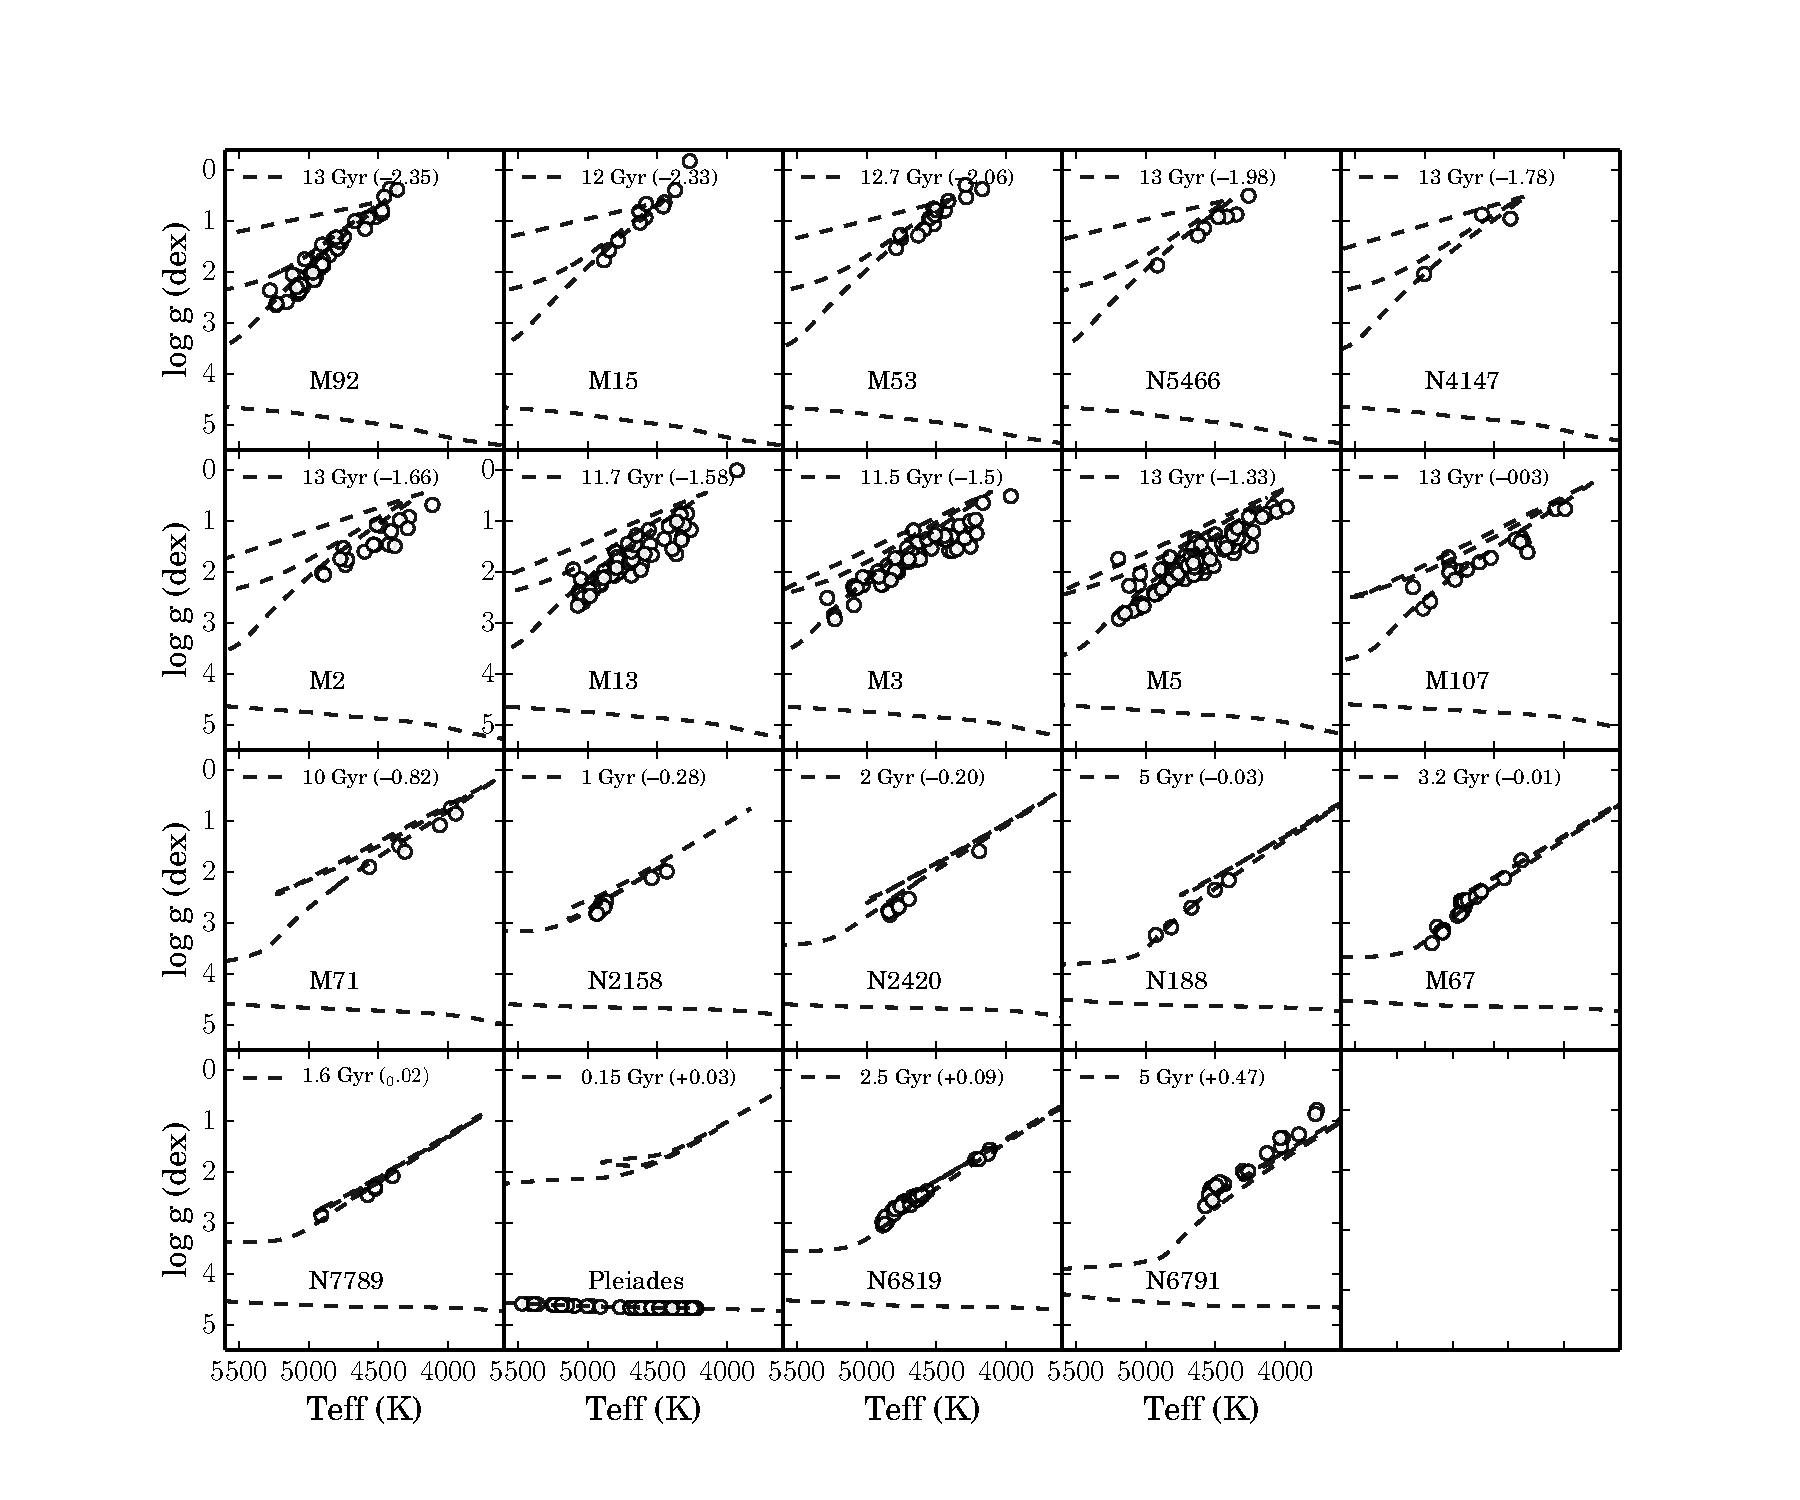
\includegraphics[scale=0.4]{./plots/training_aspcap.pdf}
\caption{\aspcap\ corrected training labels. All labels adopted from DR10 except for the Pleiades, where we implemented our own correction. }
\label{fig:trainingaspcap}
\end{figure}

\begin{figure}[h!]
\centering
  \includegraphics[scale=0.4]{./plots/training_mkn.pdf}
\caption{Isochrone-corrected \logg\ training labels: \teff\ and \feh\ labels are adopted from DR10 and the \logg\ labels are taken from vertical shifts to the isochrone. }
\label{fig:trainingisochrone}
\end{figure}


\section{Spectral Model}
\label{sec:spectralmodel}

The model is that the observed, continuum-normalized spectrum, at each
wavelength, can be explained as a linear combination of real-valued
``labels'', or a linear combination of functions of those labels.
Here the labels will be things like effective temperature $\teff$,
logarithmic surface gravity $\logg$, and metallicity $\feh$.
Additionally, the model is that at each wavelength, the observed
spectrum will deviate from the linear combination by some additive
noise contribution, some of which comes from photon noise and
sky-subtraction noise and other instrumental contributions, and some
of which is an intrinsic scatter, presumed independent at each
wavelength.
The model is built using ``training data'' (with known labels) and then
used to tag (or infer labels for) the ``test data''.

In the training data there will be $N$ spectra $n$, each of which has
a continuum-normalized flux measurement $f_{n\lambda}$ at wavelength
$\lambda$. Each of the training spectra $n$ has $K$ labels $\boldsymbol{l_{nk}}$, each of which
is (for now) presumed to have negligible uncertainty and contained within a label vector $\boldsymbol{x_n}$.

The general model is
\begin{eqnarray}
f_{n\lambda} &=&
\boldsymbol{\theta_\lambda}^T \cdot \boldsymbol{x_n} + \mbox{noise}
\
\end{eqnarray}

Where the flux $f_{n\lambda}$ of each spectra at every pixel is a general function of the labels which predict the spectrum given some noise, where $\boldsymbol{x_n}$ is some (possibly complicated) function of the full set of $K$ labels, $\set{l}_n$, which is is a vector or blob of the $K$ labels for spectrum $n$ and $\set{\theta}_\lambda$ is the set of parameters controlling the function $\boldsymbol{x_n}$ that determines the flux, at each wavelength.
%%

The simplest spectral model is that in which the function $\boldsymbol{x_n}$ is
linear in the labels, so this label vector is described as:
\begin{eqnarray}
\set{x_n} =  [1, l_1 - \bar{l}_1, l_2 - \bar{l_2}, l_k - \bar{l_k}, .. ] &\equiv& [l_{n1}, l_{n2}, \cdots, l_{nK}]
\end{eqnarray}.

The $\mean{l_k}$ are offsets (possibly means of the training data) to keep the model ``pivoting'' around a reasonable point in tag space.


Our general model then becomes
\begin{eqnarray}
f_{n\lambda} &=&
g(\boldsymbol{l_n} |  \boldsymbol{\theta_n}) + \mbox{noise}
\label{eq:linear}
\end{eqnarray}

Where the noise is a rms combination of the associated uncertainty variance
$\sigma_{n\lambda}^2$ of each of the pixels of the flux from finite photon counts and instrumental effects and the intrinsic variance or scatter of the model at each wavelength of the fit, $s_\lambda^2$. We assumed that the noise is Gaussian, zero mean, and independent for every measurement and the noise model is $\mbox{noise} = [s_\lambda^2+ \sigma_{n\lambda}^2]\xi_{n\lambda}$, where $\xi_{n\lambda}$ is a Gaussian random number with zero mean and unit
variance.

If there are missing flux values in the training data, these can be
handled by setting variances to something very large (or inverse
variances to something very small).

This model leads to the single-pixel log-likelihood function 
\begin{eqnarray}
\ln p(f_{n\lambda}\given\set{\theta^T}_\lambda, \boldsymbol{x_n}, s_\lambda^2) &=&
 -\frac{1}{2}\frac{[f_{n\lambda} - \set{\theta}_\lambda \cdot \set{x_n}]^2}{s_\lambda^2 + \sigma_{n\lambda}^2}
\label{eq:like}\\
\quad.
\end{eqnarray}


The vector $\set{f}_\lambda$ is the set of spectral flux values for
the $N$ objects all at wavelengths $\lambda$.
We can set the parameters $[\set{\theta}_\lambda,s_\lambda^2]$ either by
optimizing the likelihood (\ref{eq:like}) or by applying priors and
performing some kind of probabilistic inference (with, say, Markov
Chain Monte Carlo techniques).
Here we will optimize for now.

In this \sectionname, we are treating the function parameters
$\set{\theta}_\lambda$ and the scatter $s_\lambda^2$ as free parameters, and the
labels in the label vector $\set{x_n}$, $l_{nk}$ as fixed.
The likelihood function (\ref{eq:like}) is presented as being a
function of these free parameters.
In the next \sectionname, the tables will turn, and we will treat the
function parameters $\set{\theta}_\lambda$ and scatter $s_{\lambda}^2$ as fixed and
the labels $l_{nk}$ in the label vector, $\set{x_n}$, as parameters.
The difference is that here we are treating the training data as
having perfectly known labels, and later we will be inferring labels for
new spectra.

Then, in training, we determine:

\begin{eqnarray}
\set{\theta_\lambda} \leftarrow \substack{\mbox{argmax}\\
{\theta_\lambda}  }
\sum_{n=1}^N \mbox{ln p}(\set{f_\lambda} | {\theta_1,...\theta_\lambda})
\end{eqnarray}

The linear-in-labels form (\ref{eq:linear}) has many useful and
excellent properties.
The first is that optimization of the model, at fixed scatter
$s_\lambda^2$ is a pure linear-algebra operation (weighted least
squares); simultaneous optimization of all the parameters
$[\set{\theta}_\lambda,s_\lambda^2]$ is only nonlinear in the $s_\lambda^2$
parameter.

%
The second is that the tag inference (label-transfer; described in the
next Section) on the test data will have a very simple form.
The third is that the coefficients $\theta_{\lambda 0}$, seen as a discrete
function of wavelength $\lambda$, can be seen as an estimate of
the \emph{mean spectrum} (provided that the offsets $\mean{l_k}$ are
the mean tag values over the $N$ training spectra); and the
coefficients $\theta_{\lambda k}$ can be seen as the mean first derivatives of
the expected spectrum with respect to each of the $k$ labels, estimated
over the range of the training data.

The (perhaps) second-simplest spectral model is that in which the
functions $\set{x_n}$ are quadratic in the labels: so this label vector is described as:
\begin{eqnarray}
\set{x_n} =  [1, l_1 - \bar{l}_1, l_2 - \bar{l_2}, l_k - \bar{l_k}, (l_1 - \bar{l_1})(l_1 - \bar{l_1}), .. ] &\equiv& [l_{n1}, l_{n2}, \cdots, l_{nK}]
\end{eqnarray}.

This quadratic-in-labels form (\ref{eq:quadratic}) is similar to and
different from the linear-in-labels form (\ref{eq:linear}) in a number
of ways.
It is still the case that optimization of the model, at fixed scatter
$s_\lambda^2$ is a pure linear-algebra operation (weighted least
squares).
However, tag inference (described in the next Section) on the test
data will no longer be simple; it will now require non-linear
optimization.

The coefficients $\theta_{\lambda 0}$ can still be seen as an estimate of the
\emph{mean spectrum} (provided that the offsets $\mean{l_k}$ are the
mean tag values); the first-order coefficients $\theta_{\lambda k}$ can still
be seen as first derivatives of the expected spectrum with respect to
each of the $k$ labels, but now evaluated at the mean spectrum; the
second-order coefficients $\theta_{\lambda kk'}$ can now be seen as mean
second derivatives of the expected spectrum with respect to pairs of
labels $k$ and $k'$



\section{Parameter estimation}
\label{sec:paramestimate}

In the previous \sectionname, we built data-driven spectral models
from training data.
These models have the property that, given labels, they can be used to
predict continuum-normalized flux, up to observational and intrinsic
scatter.
In this \sectionname, we are going to solve the inverse problem; we
are going to presume that we have spectra, but we don't have labels.
In this case, we will use inference to obtain labels for the untagged
spectra.
These untagged spectra will be referred to as the ``test data'' in
what follows.

In the test data there will be $M$ spectra $m$, each of which---as in
the training data---has a continuum-normalized flux measurement
$y_{m\lambda}$ at each wavelength $\lambda$, and an
associated observational uncertainty variance $\sigma_{m\lambda}^2$.
Again, if there are missing flux values in the test data, these can be
handled by setting variances to something very large.
The difference between the training data and the test data is that the
test data do not (yet) have known labels $x_{mk}$; we are going to infer
these.

Just as in the previous \sectionname, our model is given in
equation~(\ref{eq:model}).
This model leads to the same likelihood function given in
equations~(\ref{eq:like1}) and (\ref{eq:like}), but this time seen as
being functions not of the function parameters $\set{\theta}_\lambda$ and
scatter $s_\lambda^2$ but instead as functions of the \emph{labels}
Then, in determining labels, we determine: 

\begin{eqnarray}
\set{l_\lambda} \leftarrow \substack{\mbox{argmax}\\
{l_n}  }
\sum_{\lambda=1}^\Lambda \mbox{ln p}(\set{f_\lambda} | {\theta_1,...\theta_\lambda})
\end{eqnarray}

where the likelihood functions are given as a function of labels now,
the sum is now over the full set of wavelengths
$\lambda$, and the vector $\set{y}_m$ is the vector of fluxes from
spectrum $m$ for all wavelengths $\lambda$.
These likelihood functions effectively assume that the function
parameters $\set{\theta}_\lambda$ and scatters $s_\lambda^2$ are all known (from
the training data).
New labels $\theta_{mk}$ for object $m$ can be obtained either by maximizing
the likelihood function (\ref{eq:taglike}), or else by applying priors
and performing probabilistic inference.
Here we will optimize for now.

When we use the simple linear-in-labels form (\ref{eq:linear}) for the
mean model $\set{x_n}$, the optimization to obtain maximum-likelihood labels
(given parameters $[\set{\theta}_\lambda, s_\lambda^2]$) is simple linear
least-square fitting.
This optimization is obtained by straightforward linear algebra on the
spectral pixels $y_{m\lambda}$, and standard frequentist confidence
intervals can be obtained similarly.

When we use the quadratic-in-labels form (\ref{eq:quadratic}) for the
mean model $Y()$, there is no simple linear-algebra operation that
optimizes the likelihood. Instead a python curve$\_$fit optimising function is used, which optimises the values for the parameters so that the sum of the squared error of f(xdata, $*$popt) $-$ ydata,  is minimized. 

We have described how we construct our model and then apply our model to get labels for new stars, We now present in \ref{sec:results} the results for our model, starting with the simplest linear first-order implementation and then for the model we used for all \apogee\ data, of the quadratic model, linear in the coefficients and non-linear in the label-inference.  For the quadratic model we then show this applied to the DR10 data, including at lower signal-to-noise and investigate different input training labels. 



\section{Results}
\label{sec:results}

We have five primary results that we report. The first is that we can demonstrate, via the scatter which we optimise, that our model is a good fit to the data. This says that our model is predictive and we perform a cross validation to assess the errors we expect for our test data, which is the DR10 \apogee\ spectra. A cross validation performed with a take-one-cluster out test however tells us that our training sample is too small, each cluster is critical to the results. We are also critically lacking in dwarf training spectra. If the Pleiades stars, which comprise the dwarfs, are removed we can not recover parameters for dwarfs and so can not differentiate dwarfs in DR10 test data. Furthermore, the training data does not cover the full parameter space of DR10 observations. Given the constrained training set however, the label-transfer method using DR10 test data is shown to work extremely well and this showcases the strength in this approach ,that with only 550 training stars, we can reproduce all DR10 labels for the stars in the \apogee\ survey, quickly and simply.  The second result is that via our method, we can use the model for determining continuum pixels, which are robust and true continuum over the label-space of the training data and this continuum normalisation is implemented for both training and test data and validated across signal-to-noise. 

The success of the method using the DR10 data is our third result. We can reproduce \textit{all} \aspcap\ DR10 labels, of \teff\, \logg\ and \feh\ with errors of \teff\ $<$ 90 K, \logg\ $<$ 0.18 dex and \feh\ $<$ 0.08 dex. The rms dispersion of \apogee - \tc\ is no larger than \apogee\ parameter errors reported in \citep{Meszaros} as our method generates insignificant errors at the SNR of the combined visit \apogee\ data. We also report results for dwarfs but these are constrained by the very limited dwarf set in our training sample, and we do not provide a robust measurement of these stars across metallicity, given our single metallicity dwarf training set. The fourth result, from the testing of the DR10 data is that objects which are not in our training data set give unphysical parameters in their labels. These objects with unphysical parameters were found to be fast rotators, which can be easily excluded using the \aspcap\ rotation warning set flag. This demonstrates that we can only be as good as our training set. The final result that we report is the performance of \tc\ at low signal to noise. We demonstrate that \tc\ returns robust stellar parameters at an SNR of $<$ 30. For this test we do not nosify the spectra but rather use the single visit spectra available in the \textit{apStar} DR10 data files. The performance of \tc\ at low SNR reflects both the success of the continuum identification and the strength in using \textit{all} of the spectral range to characterise the labels by allowing the regression to determine which pixels control the labels themselves.



\subsection{The model} 

To firstly evaluate the label-transfer method, we performed the simplest implementation of a first-order linear model comprised of four coefficients. Figure \ref{fig:self1} shows the performance of this model for the 550 stars in the training set, run back through \tc\, having used the very same stars to set the coefficients for the model. The bias, rms and precision represent the offset and difference between the input and output labels and the internal error of the label inference, respectively. The model is clearly too inflexible to describe the behaviour of flux with the labels. This is not surprising given it is known that absorption features and particularly strong lines, do not behave linearly to the first-order, as a function of stellar parameters. Different metallicity regimes show different trends in  temperature and \logg\ and the dwarf labels are not well reproduced, showing large scatters in the \logg\ and \feh\ labels. 

The linear model can be vastly improved by selecting only weak line regions, and excluding all strong lines by implementing a cut on the normalised flux considered for the coefficients fit in the label transfer. The loss of information in the exclusion of a significant fraction of pixels is however clearly suboptimal. 

\begin{figure}[h!]
\centering
  \includegraphics[scale=0.55]{./plots/single_self.pdf}
\caption{The performance of the label-transfer of \tc\, where input coefficients have been determined using the set of training stars then run back through \tc\ as test data, to determine how the model can predict their labels; a test of the ``goodness'' of the model, for the simplest linear case with four coefficients. }
\label{fig:self1}
\end{figure}


The perhaps the second simplest model we can implement, is the quadratic model, with ten coefficients describing the labels, (\ref{eq:linear}).  Overall, this model describes the behaviour of the flux with the labels across their parameter space fairly well and is clearly significantly better than the first-order linear model within the parameter range of these stars. 

The results for the first-order coefficients and the scatter of the fit for the quadratic-in-labels model, is shown in Figure \ref{fig:coeffs}, across a narrow region of the spectra. The top panel shows the scatter of the fit, indicating the dispersion of the flux of the training data around the model at each pixel and the mid-panel corresponds to the intersect of the model of the training sample, with regions of first order label dependence shaded in the different colours corresponding to \teff, \logg\ and \feh. The bottom panel shows the first order coefficients $\theta$ in \teff, \logg\ and \feh\.  The scatter is small and this indicates that our model is a good representation of the data. From this intersect flux, the continuum pixels have been determined, which  are then used for the final continuum normalisation for the stars, both training data and test data. 

 In the bottom panel of Figure \ref{fig:coeffs}, the red, blue and green shaded regions show the highest 2$-\sigma$ coefficient values in the \feh, \teff\ and \logg\ labels respectively. These regions indicate where these flux levels are strongly proportional to these labels and highlights the differences between the labels in their flux dependancy. Note there are many regions where the \feh\ label dominates in contribution to the flux. From the bottom panel of Figure \ref{fig:coeffs}, it is clear that there is significant covariance between the labels and the \logg\ label has the weakest first-order dependence on the flux of the three labels across this sample wavelength interval. 

By returning coefficients, we have a tool which describes the flux in a quantitative way as a function of stellar labels, thus removing degeneracies and improving the prospects for determining stellar parameters, by modelling covariance rather than minimising it. We discuss this in section [DWH this is where you write the quantitative thing you and HW talked about in the forest ??].

For the overall label profiles in the middle panel of Figure \ref{fig:coeffs}, there is typically asymmetry for a given absorption feature, in the flux and the labels. There are very few regions were the flux is a function of only one of the labels, and pixels are typically covariant. The strongest \logg\ dependence is typically associated with weak lines and the \teff\ and \feh\ labels, with strong lines. 

 
 %made with run -i makeplot_scatter_test18_step.py
\begin{figure}[h!]
    \includegraphics[width=\hsize]{./plots/R1_continuum2.pdf}
  \caption{Top panel: the scatter of the fit, middle panel: the mean spectra from the first coefficient, from the training set and the bottom panel; the first three coefficients ($\theta_1$, $\theta_2$, $\theta_3$),  which correspond to the first-order label terms ($\teff, \log, \feh$). In the mid panel the yellow pixels points are the selected continuum pixels from the coefficients and continuum returned by the model.  The red, blue and green points show the highest 2$-\sigma$ coefficient values in the \feh, \teff\ and \logg\ labels respectively. This indicates where these flux levels are strongly proportional to the labels. Note the \feh\ label is dominant in the contribution level and from the bottom panel it is clear that there is significant covariance between the labels and lesser regions of strong \logg\ dependence, across this sample wavelength interval.}
\label{fig:coeffs}
\end{figure}
- QN  - Do I have to somehow normalise these values by diving by their std or range ? 


To assess the uncertainty of our model, we perform a take-one-cluster out test and a take-one-star out test. . For the take-one-cluster out test we train the model iteratively on all clusters except for an excluded one, and then run the removed cluster through the label-transfer, to see how well the model can predict labels for the cluster stars. Similarly, for individual stars.  

Figure \ref{fig:takeoneout} shows the cross-validation results for take-one-cluster out test. This Figure demonstrates that each cluster is critical to the training set and removing even one is extremely detrimental to the model. This sensitivity indicates that he model is significantly too small and certainly sub-optimal. We can only do better by expanding on this most basic model. Additionally, for the take-one-cluster out test, if the training set does not include the cluster with dwarfs, the Pleiades, then these stars are not recognised as dwarf stars. This set of dwarf training data is therefore essential to recognise dwarfs and discriminate them from giants, which is important in our running through all of the DR10 spectra. There are limitations however in this dwarf discrimination, in that not all spectral types observed as part of DR10, namely hot dwarfs with rotation, are included in our model and we can discriminate these stars based on their returned labels, but can not return correct labels for these stars. 


Figure \ref{fig:takeonestar} shows the cross-validation results for take-one star out. The single dwarf clusters shows the poorest self-determination, particularly in the \feh\ labels. 


The results for the bias and rms are indicative of how well our model performs over the full , and these will inherently include the uncertainties on the input labels (from ASCPAP corrected values, of \teff $<$ 150 K, \logg $<$ 0.2 dex and \feh\ $<$ 0.1 dex \citep{Meszaros2013}. There are outliers, and certain cluster members, M3 and M5 and stars in M13 in particular, seem grouped together, offset in \teff\ and \logg\ space. 

Removing these clusters improves the \teff\ and \logg\ rms by 10\%. The rms is comparable and less than the estimated \apogee\ errors with \logg\ performing the most over the \apogee\ estimates.  

The outlying stars may be due to an anomalous scale of the input labels of these stars compared to the other training data, or it may be due the nature of the spectra of these stars, that is not accounted for in the model. Similarly, the temperature of the dwarfs is offset low at increasing temperature, compared to the input labels, so the model may be limited in describing the difference between dwarf and giant spectra. The labels perform best in [Fe/H] space, which may not be surprising given the information content in the [Fe/H] coefficient described in section \ref{sec:results}. However, there is a flattening at the low metallicity end of the model in \feh\ in the output labels at \feh\ $<$ -2.2. 






\begin{figure}[h!]
\centering
  \includegraphics[scale=0.55]{./plots/quad_takeoneout.pdf}
\caption{Take-one-cluster-out test.}
\label{fig:takeoneout}
\end{figure}

\begin{figure}[h!]
\centering
  \includegraphics[scale=0.55]{./plots/takeonestarout.pdf}
\caption{Take-one-star-out test.}
\label{fig:takeoneout}
\end{figure}

-- What do we say about all of this. 

-- may be due to incorrect input labels, inconsistency of input labels. ?

-- They show... departures from linearity... outliers... is it really a better model?..

...what are we doing about outliers?  If anything?  Perhaps in discussion too... = just leaving them there nothing. 

- discuss how this method can be improved using priors as have this information e.g know space in Teff-logg that stars should lie in. 

...is this a good model?  No; how do we know? - well it beautifully reproduces ASCAP labels although looks a bit scattered in self test.


\begin{table*}
\centering
\caption{Excerpt of table of measured stellar parameters from label transfer of \tc\. The full table of 42,000 stars is available online. We include DR10 commissioning fields for which no ASPCAP parameters were available and for these stars, marked with $^1$ we do not exclude on \textit{rotation warning flag set}. The full table is available as Supplementary Material online.}

\begin{tabular}{| c | c | c |  c | c | c |  c | c |}
\hline
star ID & \teff\ & \logg\ & \feh\ & \teff\mbox{$_err$} & \logg\mbox{$_err$} & \feh\mbox{$_err$} & $\chi^2$\\
{2MASS} &  K &  dex  & dex & K & dex & dex & \\    
\hline
-- &    -- &      -- &      -- &    -- &   -- &     -- & -- \\
-- &      -- &    -- &      -- &    -- &   -- &    -- & -- \\
-- &      --&     -- &    -- &    -- &     -- &     --&  -- \\
-- &    -- &      -- &    -- &    -- &   -- &    --&  -- \\
-- &     -- &    --&      -- &    -- &    --&      -- & -- \\
 \hline
\end{tabular}
\label{tab:online}
\end{table*}  

\subsection{Continuum Idenficiation}





These continuum pixels have been determined from the quadratic model using a combination of the flux level and the coefficients returned.  From the intersect-flux returned in the first coefficient, 35\% of the pixels across this wavelength region have a pixel level within 1\% of flux = 1. However, regions where the intersect-flux is $\sim$ 1 are not representative of continuum for all stars in the training set, e.g. metal rich stars. It is insufficient to select on pixels that are simply near the intersect-flux in isolating continuum regions. Instead, we are informed by the coefficients of the fit, and a set of coefficients which are near 0, is indicative of a pixel region where there is no dependence, or negligible dependence of the flux on the labels, across all of the training spectra. We make a final continuum selection taking the 15\% of pixels with coefficients nearest 0, for each coefficient and a flux selection of within 1.5\% of 1 (i.e. 1 $\pm$ 0.15). This criteria returns around  7\% of pixels, which we adopt as true continuum pixels for data that spans the parameter range of the training set. We use the inverse variance weighting of these pixels for the corresponding Chebyshev fit which we find to be a robust continuum normalisation across the stars that are within the parameter range of the training set, across all signal to noise. The continuum pixels are marked on sample spectra from the training data, across the metallicity regime of most metal-poor to most metal-rich cluster in Figure \ref{fig:cal_feh}.




% made with  makeplot_scatter_test18_coeffs.py
\begin{figure}[h!]
  \includegraphics[width=\hsize]{./plots/3training.pdf}
\caption{Three stars from the training data: top M92 (\teff\ = 4995 K, \logg\ = 2.1 dex ,\feh\, = -2.2 dex) middle = M5 (\teff\ = 4302 K, \logg\ = 1.4 dex, \feh\ = --1.25 dex), bottom panel: N6791 (\teff\  = 4495 K, \logg\ = 2.3 dex, \feh\ = 0.4 dex. \textbf{Need to improve continuum normalisation so first panel does not look like first panel currently does}. }
\label{fig:cal_feh}
\end{figure}




\subsection{Anomalous Spectra: Dwarfs and Rotation}

The dwarf spectra in our training set consists of the Pleiades cluster, at a single metallicity. This restricted sample constrains our ability to determine the stellar parameters for dwarf stars. Given these training data, our model \textit{can} differentiate dwarfs from giants, as long as their spectra is comparable to that of the Pleiades. However, none of the dwarfs in our training set are hot rotating objects, with broad line features, for example the stars in Figure \ref{fig:dwarfs}, which comprise a fraction of \apogee\ DR10 data. 

It is possible to differentiate these stars with \tc\, as they are output in non-physical space in \teff-\logg, and present as a group of very metal poor, \feh\ $\sim$ --2.0, low \logg\ stars $\sim$ 0, with cool temperatures $\sim$ 4000 K. The metal poor solution determined by \tc\ reflects the dearth of lines in the spectra for these hot stars, given the training model. 

This group of stars is flagged in \aspcap\ with a ROTATION WARNING flag set. We therefore are able to exclude these stars from our analysis using this condition. 
 
 % made with  makecontin_data_dwarfs_split.py
 \begin{figure}[h]
 \includegraphics[scale=0.5]{./plots/dwarfs.pdf}
  \caption{Examples of hot rotating dwarfs in the \apogee\ DR10 data which are not included in our training data; we can not determine stellar parameters for these stars as they are not captured in our model.}
\label{fig:dwarfs}
\end{figure}

\subsection{DR10 Comparison}
 
We have run \tc\ through all stars in DR10 contained in both the \textit{aspcapstar} files,  which comprise about 46,800 stars, in 150 fields and an additional 4800 stars in 20 commissioning fields available in the \textit{apStar} files\footnote{These were excluded from final figures as the rotation warning flag is set for all of these stars}, for a total of $\sim$ 51,600 \apogee\ DR10 stars. The comparison of \tc\, showing the bias, rms and precision for 6 sample fields, with bulge, disk and halo targeting are provided in Figure \ref{fig:cal}. We reproduce the \aspcap\ corrected stellar parameters extremely well. In addition, we also return a fraction of dwarfs (not shown in these Figures as \apogee\ does not report ASCAP corrected dwarf parameters for DR10). 
%We are able to exclude dwarfs with large rotation, for which we can not measure the labels. 

\begin{figure}[h!]
\centering
  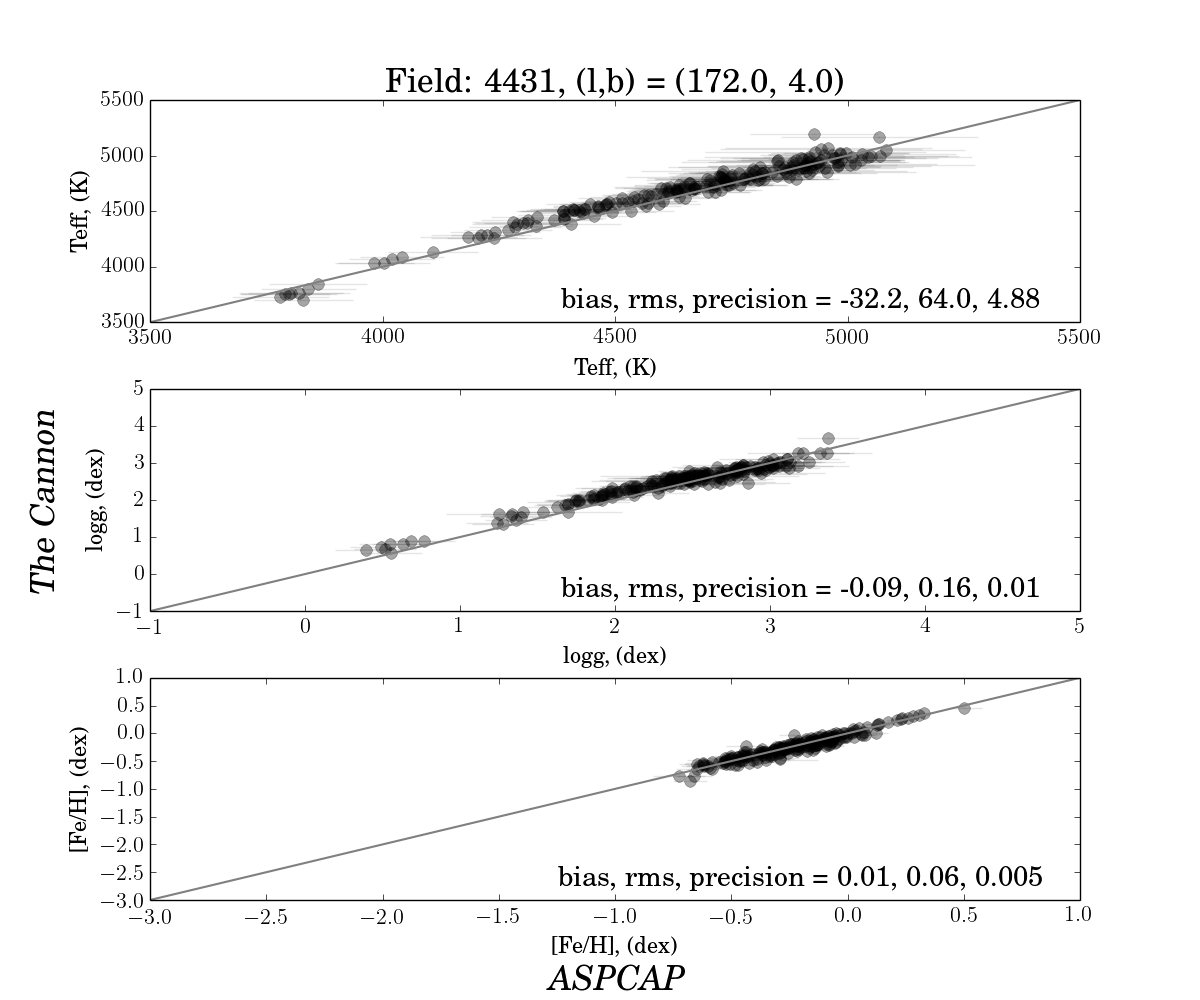
\includegraphics[scale=0.25]{./plots/4431_v19.pdf}
    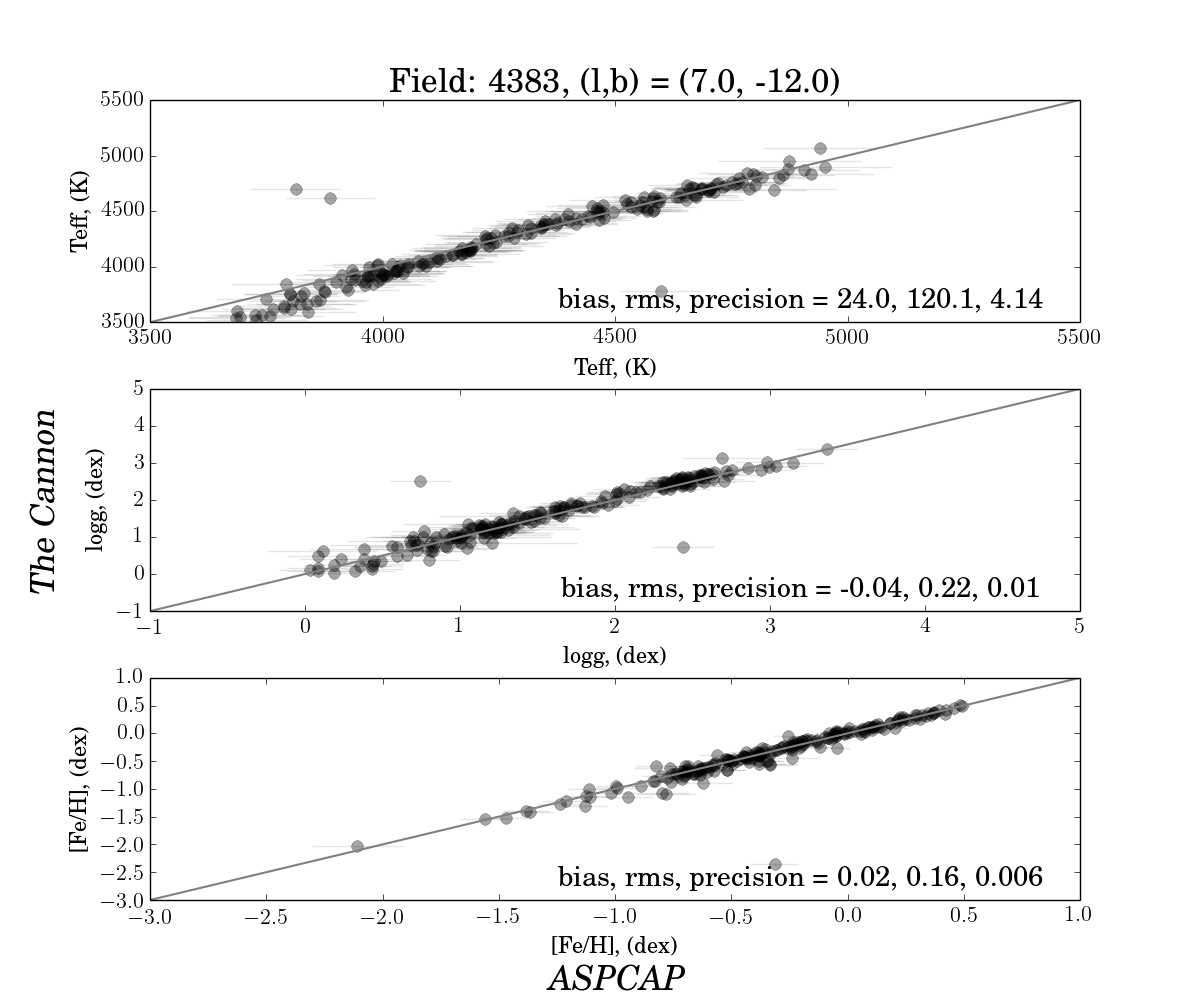
\includegraphics[scale=0.25]{./plots/4383_v19.pdf} \\
      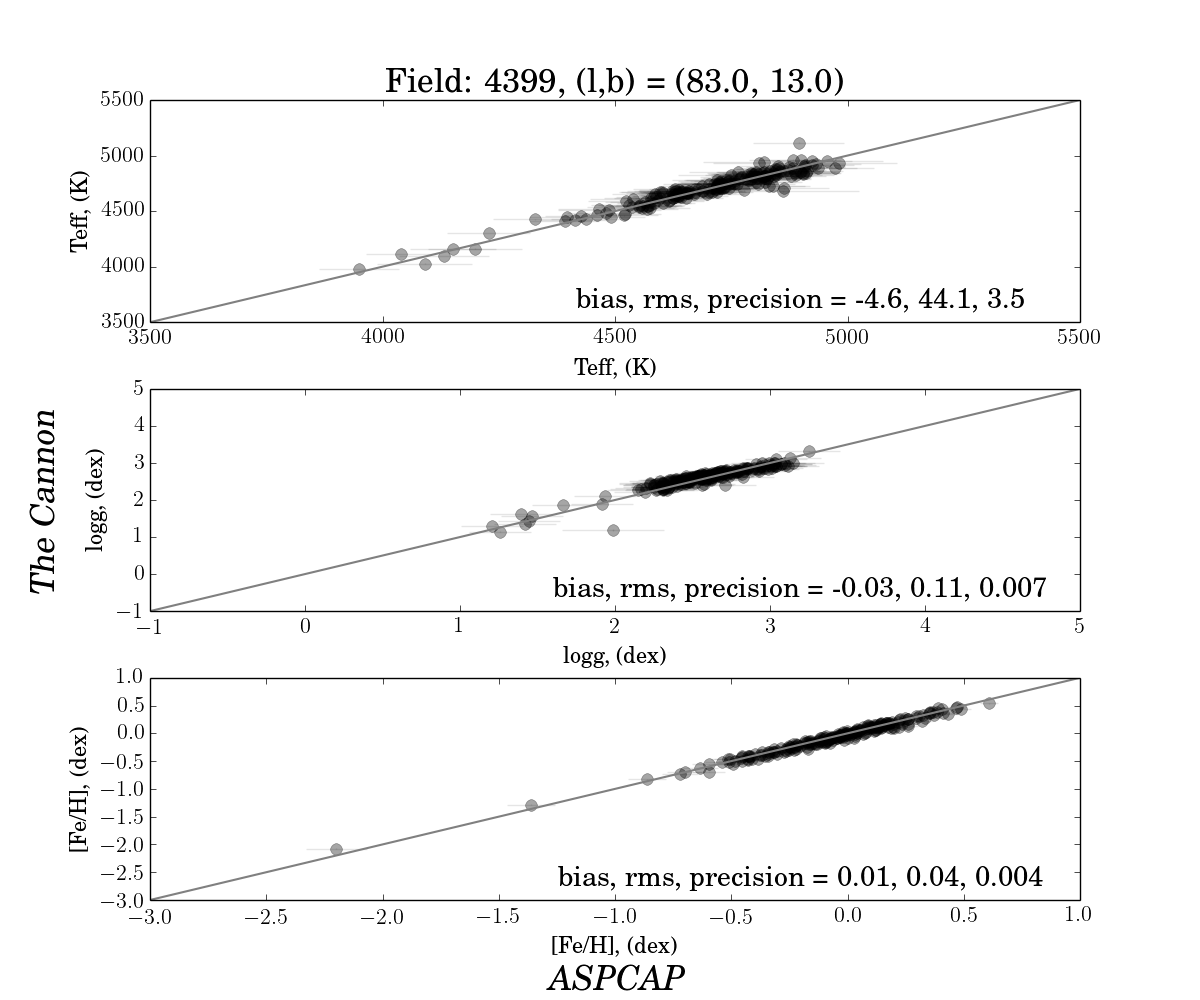
\includegraphics[scale=0.25]{./plots/4399_v19.pdf}
        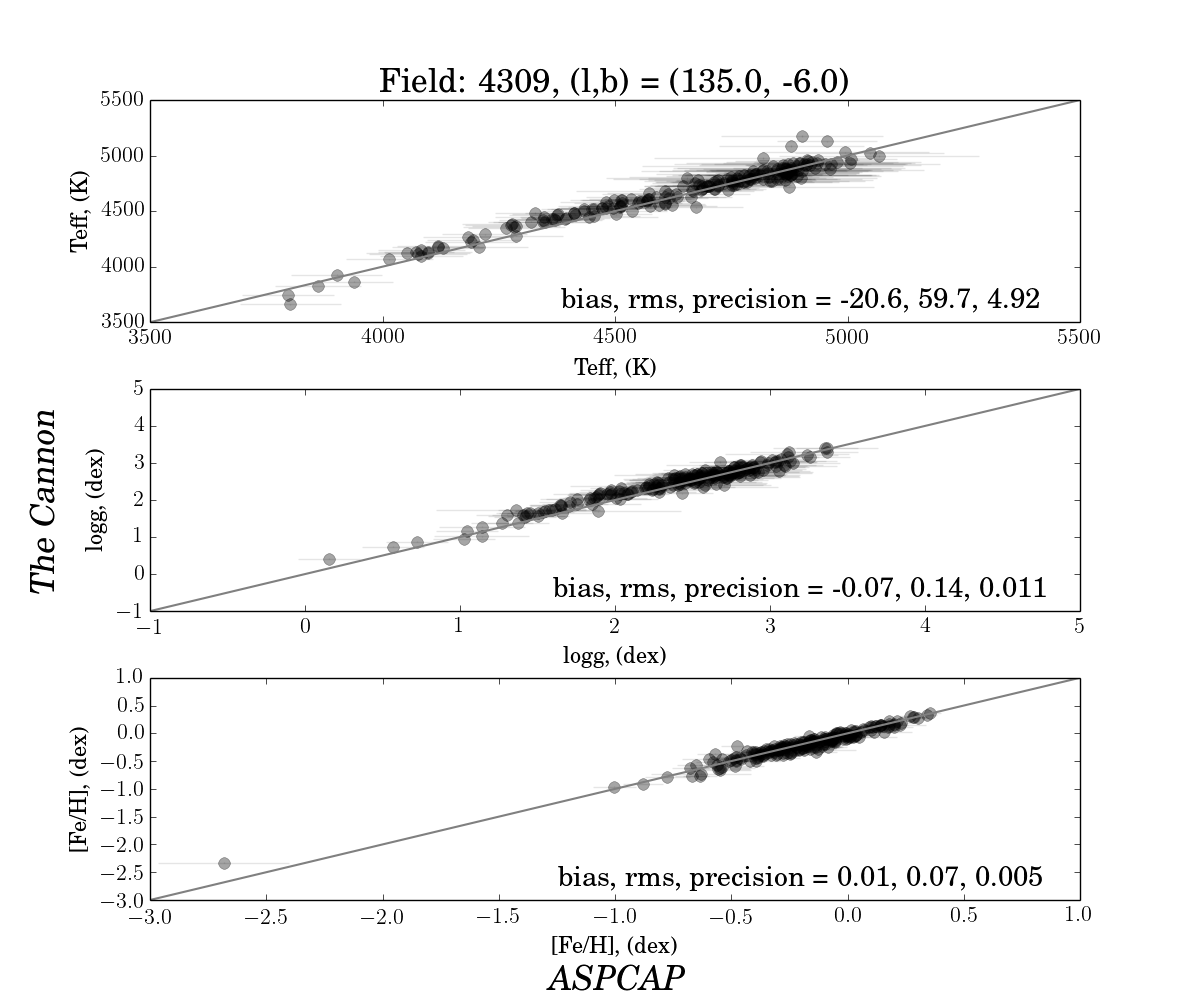
\includegraphics[scale=0.25]{./plots/4309_v19.pdf} \\
              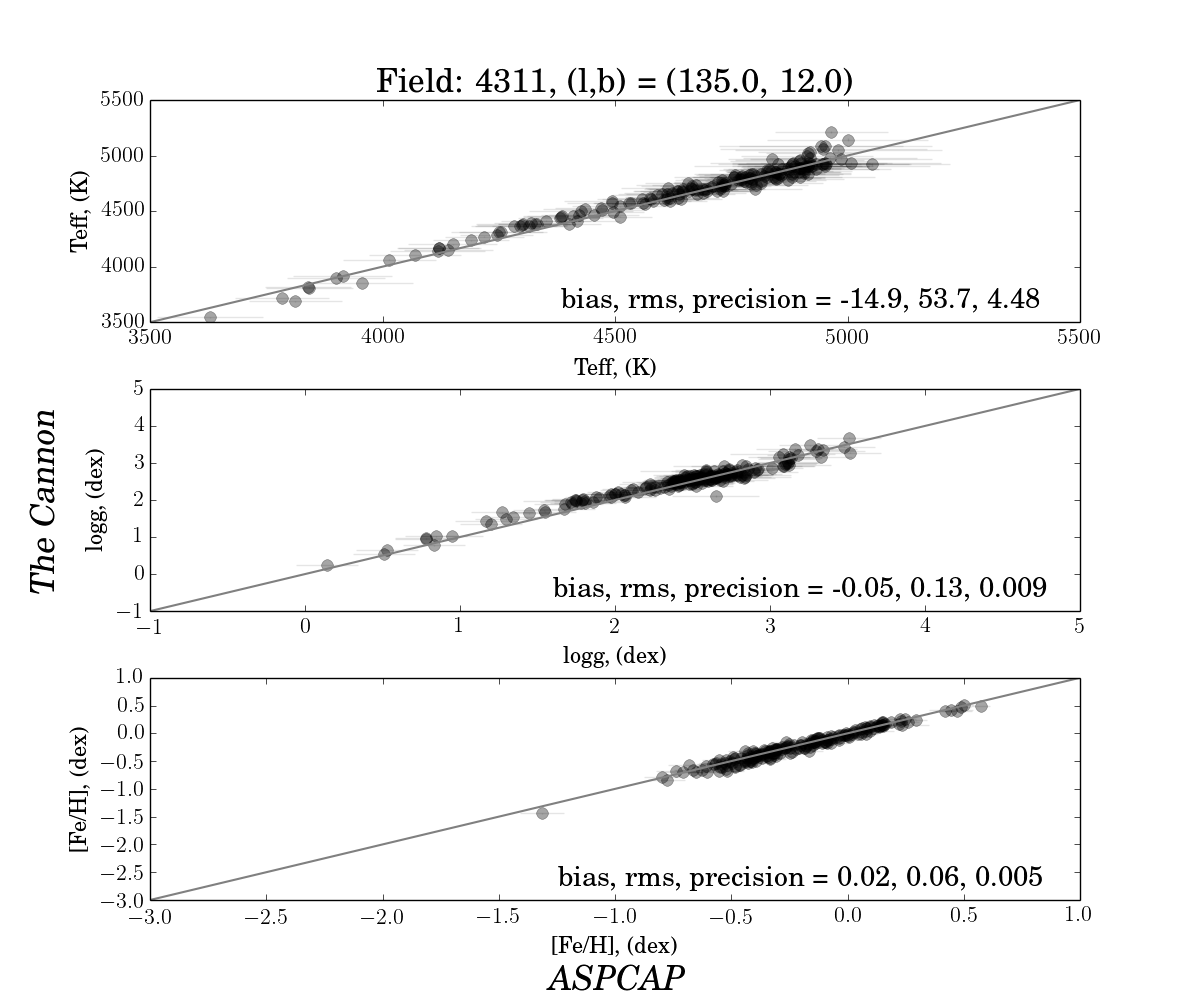
\includegraphics[scale=0.25]{./plots/4311_v19.pdf}
        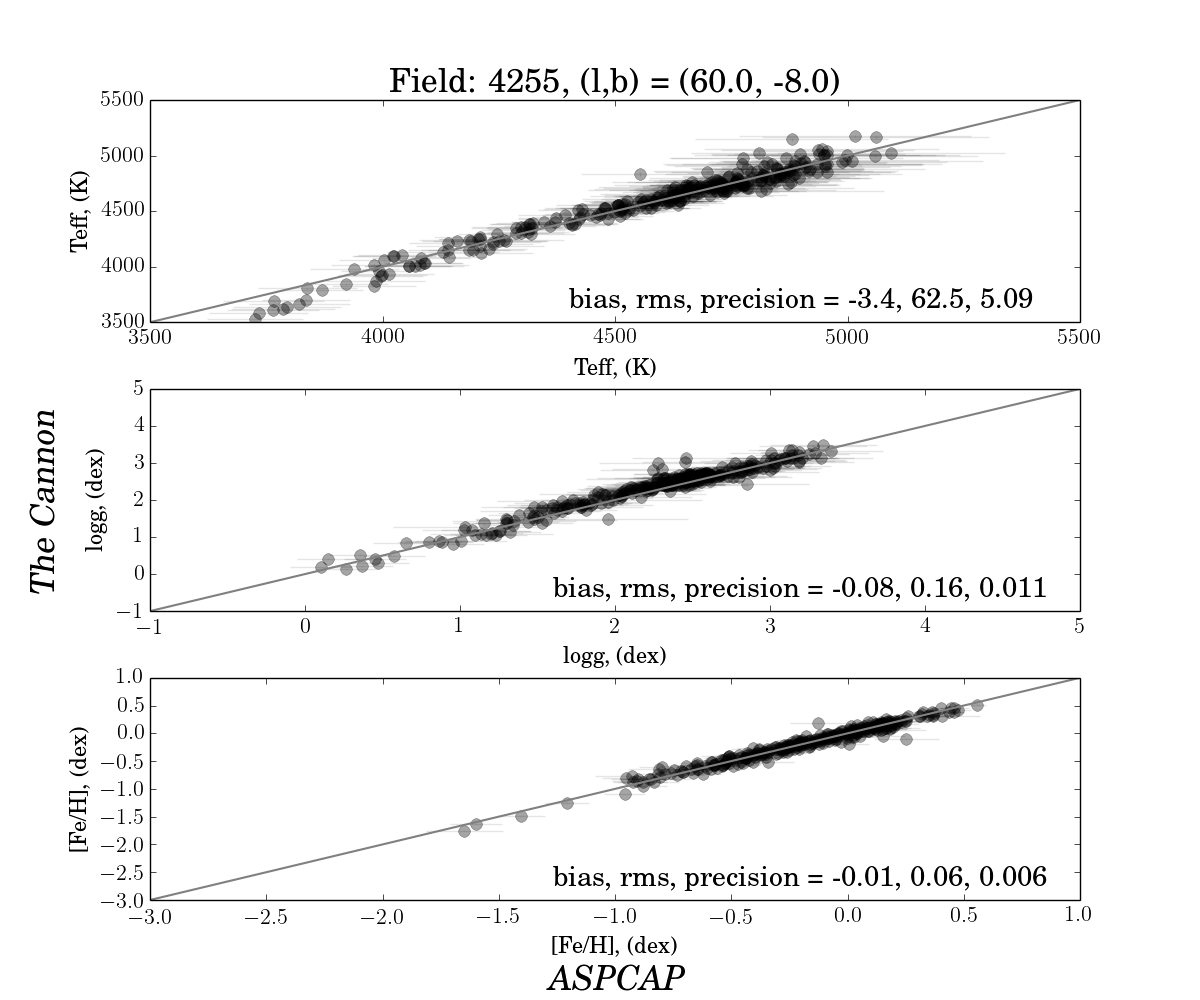
\includegraphics[scale=0.25]{./plots/4255_v19.pdf} \\
\caption{\small{\aspcap\ DR10 versus \tc\ for 6 different fields including in the disk, bulge and halo}}
\label{fig:cal}
\end{figure}


The results of \tc\ for DR10 stars compared to \aspcap\ is shown in Figure \ref{fig:DR10_compare}. These panels show the individual stars and density contours  (minimum 300 stars, maximum 1000 stars), for the 30,500 stars that have stellar parameters in \textit{ASPCAP}. There are very small offsets between \tc\ and \aspcap\ of +12 K in \teff\, -0.04 dex in \logg\ and +0.01 dex in \feh\. The rms error of this comparison of 87K in \teff, 0.18 dex in \logg\ and 0.08 in \feh\ is comparable to the error estimates for \apogee\ parameters in \citet{Meszaros2013} of 150 K in \teff\, 0.2 dex in \logg\ and 0.1 dex in \feh.  The typical internal precision on the measured parameters from \tc\ is 5.6 K in \teff\, 0.01 dex in \logg\ and 0.006 dex in \feh\ 

- note these errors are divided by dof need to properly understand these. \\

-note should cut on chis



We show the location of the stars in the \teff-\logg\ plane from \tc\ for the stars in DR10 in Figure \ref{fig:test18}. There are 37,500 stars in this plot which are remaining stars after excluding stars with the  rotation warning flag set, with velocity scatter $>$ 10 \kms and telluric calibration target set. For approximately 14\% of these stars, we return dwarf parameters for, with \logg $>$ 4 dex.  The stars that have been determined using targeting flags and inspection of the spectra, to be dwarfs with rotation, lie in an unphysical space at very low \feh and log g and have been removed using the \aspcap\ rotation warning set flag and this is a limitation of the training sample. 
%From our total of  51,600 stars, then cut down to 39,500 after cutting out  the approximately 7500 stars with

Although we find excellent agreement between \tc\ and \aspcap\ by adopting ASCPAP corrected labels and additionally are able to derive parameters for dwarf stars in DR10, the \teff-\logg plane for these stars shows an unphysical narrow giant branch  (see Figure \ref{fig:test18}). The narrowness of the giant branch is however directly a consequence of the input labels of the training spectra. 

%Tests on the input labels to \tc\ demonstrate that there is practically no difference to the output results from adopting individual [Fe/H] values for the stars (i.e. from the \aspcap\ corrected values) or else a single [Fe/H] value for every star in a cluster, using the literature value of the cluster.

\begin{figure}[h!]
  \includegraphics[width=\hsize]{./plots/isochrone_v19.png}
\caption{test18}
\label{fig:test18}
\end{figure}

The results using our alternative log g calibration described in \sectionname{} remove our results slightly from the \aspcap\ scale in each of the parameters. However, with these new \logg\ labels, we find a broad giant branch width that is consistent with expectations in \teff-\logg\ space given the metallicity of these stars. The \teff-\logg\ plane for this alternative calibration is shown in \ref{fig:mknA}. Figure \ref{fig:iso_density} demonstrates the density contours for the stars in the DR10 release returned with \tc\, showing the expected red clump. 

%The most dramatic difference is that the giant branch width from DR10 stars is consistent with the distribution in [Fe/H]. There is now excellent agreement with the isochrones for all DR10 to very low gravities. 

Using our own calibration of the \logg\ values, we also find good  good agreement with Kepler \logg\ values. The difference between Kepler and \tc\ \logg\ values is also \teff\ independent, which is not the case for training on the \apogee\ labels. This is discussed in Section \sectionname{}.  


\begin{figure}[h!]
  \includegraphics[width=\hsize]{./plots/isochrone_mknA.png}
\caption{Training labels using own labels in \logg\ : moved to isochrone}
\label{fig:mknA}
\end{figure}



 \subsection{Performance at low signal to noise}

By identifying 'true' continuum pixels we have a continuum normalisation that is robust across low and high signal-to-noise (SNR). To examine how \tc\ performs at lower SNR, we have taken individual visits from the apStar fits files, when there are $\ge$ 4 visits, and using a single visit spectra. Figure \ref{fig:lowsnr} shows a comparison of a sample star for a single visit and combined visits ($>$ 4 total visits) showing the continuum normalisation works well for both of these regimes. The corresponding SNR measurement for this test,  showing SNR results binned  across SNR 5 - 200 are shown in Figure \ref{fig:SNR}.  At the highest SNR (and \apogee\ estimates a upper noise floor of 200 although stars do measure above this), the rms difference between \tc\ and \aspcap\ is comparable to the \aspcap\ measurement errors, at 73K in \teff\, 0.18 dex in \logg\ and 0.11 dex in \feh.  At a SNR of 20-50, the rms error increases to 130 K, 0.3 dex and 0.15 dex in \teff, \logg\ and \feh\, respectively. At an SNR of 0-20 the rms error is significantly higher at 220 K in \teff\,, 0.5 dex in \logg\ and 0.27 dex in \feh. The internal errors of \tc\ become comparable to typical minimisation methods in the SNR bin of 20-50 and even in the 20-30 bin only marginally exceed them. With this method we can return stellar parameters of \teff, \logg, \feh\ to as good a precisions as minimisation techniques ( \teff\ $<$ 100K, \logg\ < 0.2 dex, \feh\ < 0.1 dex) with an SNR of $\sim$ 30. 

 - need to understand errors better. 
 
 
\begin{figure}[h!]
  \includegraphics[width=\hsize]{./plots/continuum_SNR.pdf}
    \includegraphics[width=\hsize]{./plots/continuum_SNR2.pdf}
  
\caption{continuum normalisation of the same star at SNR of 120 (top) and 25 (bottom) }
\label{fig:lowsnr}
\end{figure}

Now step through, selected where $\ge$ 4 visits, taking the 4th visit and running through this. SNR results are in fig \ref{fig:SNR}

 \begin{figure}[h!]
 \includegraphics[scale=0.24]{./plots/SNR100to200c.png}
\includegraphics[scale=0.24]{./plots/SNR50to100c.png}\\
\includegraphics[scale=0.24]{./plots/SNR20to50c.png}
\includegraphics[scale=0.24]{./plots/SNR20c.png}\\
\includegraphics[scale=0.24]{./plots/SNR10to15.png}
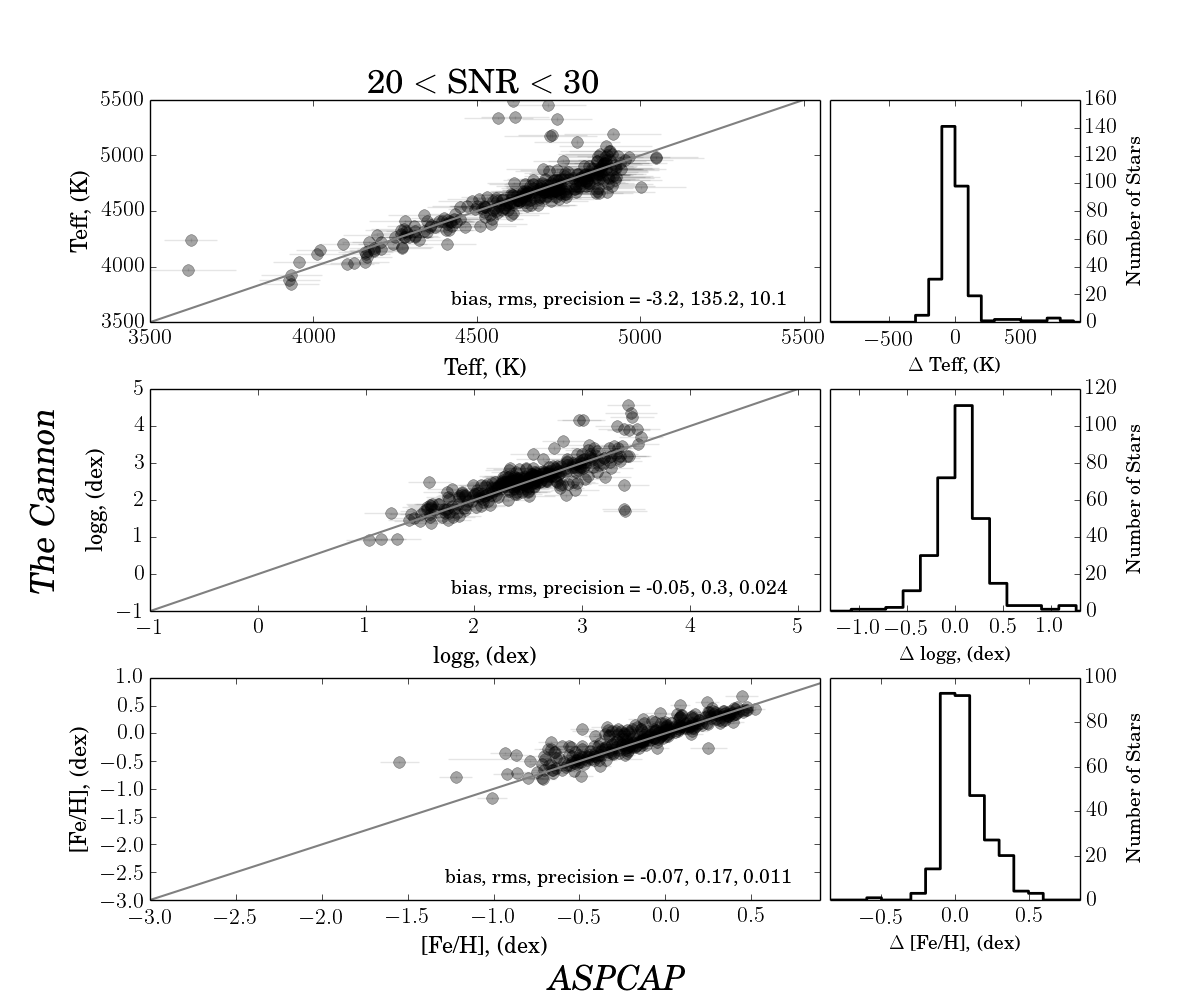
\includegraphics[scale=0.24]{./plots/SNR20to30.png}
  \caption{Four regimes of signal to noise for single visit spectra. There are 642 stars in the SNR $\le$ 20 figure, 3533 stars in the 20 $<$ SNR $<$ 50, 1211 stars in the 50 $<$ SNR $<$ 100 figure and 695 stars in the100 $<$  SNR $<$ 200}
\label{fig:SNR}
\end{figure}


\subsection{Comparison to Kepler Gravities}

We compare the results for \logg\ from \tc\ with the gravities from apokasc, where extremely precise \logg\ values have been determined for a subset of about 2000 stars using astroseismology. For the results from \tc, we find a higher scatter in our \logg\ label compared to Kepler gravities than \textit{APOGEE}, by about 15\%, but, dissimilarly to the \apogee\ log g comparison, we do not find a dependence of the gravity different on temperature. For training labels taken from our own \logg\ calibration, set to the isochrone scale, we also find a lesser separation of red giant and red clump, in the blue and red points respectively in Figure \ref{fig:kepler}. The dispersion in \tc\ \logg\ values as shown in Figure \ref{fig:kepler} is $\sigma$ = 0.16 compared to $\sigma$ =  0.14 for \textit{APOGEE}, and there is a small offset of -0.025 dex in the mean. 

That our dispersion in \logg\ is higher than \apogee\ may not be surprising given the restricted range of \logg\ values in our training set as a function of \teff\ and \feh. That there is no trend in \logg\ with temperature may indicate some deviation of stellar models and data, given our model is from data and \apogee\ employs a synthetic stellar grid. The lesser separation of red giant stars and red clump stars when training on our own labels may indicate some problem with the ab initio adopted \logg\ corrected values to the Kepler scale from the \aspcap\ calibration in DR10.

  \begin{figure}[h!]
 \includegraphics[scale=0.3]{./plots/TheCannon_Kepler_pixtest4.png}
  \includegraphics[scale=0.3]{./plots/APOGEE_Kepler.png}
 \caption{Kepler log g versus Cannon and \aspcap\ versus Kepler. Blue are red giant. Red are red clump.}
\label{fig:kepler}
\end{figure}


Ideally we want to train on Kepler stars, but may only want to train on \logg as other labels not well known and this implementation is discussed further in the discussion section. 


\section{Discussion}

- \textit{something which worries me is although it comes across in Meszaros 2013 that the SNR of 70 is required for their stellar params to quoted accuracy, it may be driven by the individual elemental abundance determination down to \feh\ of --2.0. \aspcap\ itself may perform as well at low SNR as this method? Have not seen \aspcap\ parameters for SNR of 10-15 for example/run on individual visits. I therefore think it's important to be careful what we say here.} \\

- We have demonstrated this simple method is extremely effective for returning stellar parameters for large surveys and is as it exploits all of the information in the spectra the internal errors are extremely small. - Anticipate exactly the same success with e.g. GALAH of this method for example given they are similarly targeting clutster members could also do this with a data driven model, to very efficiently return stellar parameters. 

- A data-driven model captures physical relationship between parameters, which may not be captured in stellar models. Potential to apply his method to understand where and how models and data diverge in detail. This is a way to understand the spectra, hence highly relevant for chemical tagging. 

- Propose this is powerful for chemical tagging. Not only for label transfer of individual elements but for identifying where the elements are contributing. For chemical tagging propose we will need to do something more detailed than measuring lots of elements and use grouping algorithms. First step is to characterise spectra and do a differential analysis of spectra in a survey, via this method we propose to do this. 

- \apogee\ case argues for lower SNR and more data - Although this can be applied at much lower SNR will be limited by number of lines in the spectra of individual elements but may be very instructive for a subset to instead get blocks of grouped covariant elements e.g. light, alpha, r- , s- process (see Ting et al., 2013).


- We were motivated to examine the calibration space of the labels given the unphysically narrow giant branch returned for DR10 data and found by adopting a calibration that shifts the stars to the nearest position on the isochrone (keeping the \teff\ and \feh\ fixed to \aspcap\ corrected values) the giant branch spread out in \teff-\logg\ space across metallicity and the agreement with Kepler \logg\ values was also found to be good. A problem with adopting the nearest position on the isochrone is that we assume the stars are first ascent giants, where as they may be sitting on the AGB branch or red clump as opposed to red giant. Nevertheless, errors small. 

- Future iterations - gaussian process, bringing in errors and training on individual labels from DR12 to see if can reproduce individual labels in the rest of DR12 data given these labels in the training spectra, via the label transfer. Will not be a function of synthetic spectra as data driven model . 

- Given as we are training on 550 stars we are doing remarkably well with our data driven model can reproduce all ASCAP labels with extremely small errors

- also tells where information is in spectra. part of better understanding of stellar spectra. 

-discuss moving to isochrone. assume first ascent giants may not always be correct

Using only 500 stars transferred the labels to 51,000 in \apogee\ survey. A subset of these removed due to rotation, high velocity scatter and calibration targets and shown results for 37,500 stars. 

- Extremely successful, fast, transferable between surveys. 

- Also possible for individual elements and to identify where information is held in spectra without first knowing via linelist

- Argues for lower signal to noise, may not obtain individual abundances this is limited but propose to group alpha, s-process, r-process, elements that are covariant (Ting 2013) may provide just as successful for understanding the MW as individual abundances with higher errors. 



Show very simple, extremely fast, can return all parameters except for dwarfs with rotation as these are not in our model. As we are using every pixels internal errors very small. Can be applied for basic parameters for all surveys but can also be generalised as for more stellar types and larger range of parameters may need a more generalised model. 

-DFM upgrade stuff. 

- cite matiesse. 

Our method is calibrated across dwarfs and giants and can return reliable stellar parameters to a SNR of a fraction of this (30\%) XXX, with an intrinsic scatter of x,y,z in \teff, \logg, \feh.

- Next step will be to add alpha - surely need much higher SNR to measure individual elements but 
I wonder at what SNR we can get alphas given as this looks pretty good at an SNR of 30 for the main parameters. It may not be able to be pushed too low for individual elements given as there may be only a few lines in the spectra of these elements but I'm wondering if we can group them into say alphas, s-process, r-process, e.g elements that tend to be covariant, as a broader brush than individual elements but still extracting information in different regimes. I'm hoping I can use DR12 data to train on these labels given these labels will apparently be present in DR12 in the training set, even if they are not absolute values, or totally "correct", they are going to nicely be able to be used to test this. 

- used to identify continuum
-fast, set up use for any wavelength region, used data-driven can be applied with spectral models. 
- used to successfully reproduce all parameters in DR10 spectra
- can get agreement with Kepler log g , scatter higher , likely need more stasr
- need expanded training set - need dwarfs more of them
- next step add alpha labels. 
-individual hard but go with groups
- proceed with survey at 50\% of SNR and can still extract information.

There are limitations of our model. A primary limitation is that it is very small, and we have only one set of stars that are dwarfs, all at the same nominal metallicity $\sim$ 0.03 (the Pleiades). 

It is possible to implement exactly the same procedure using a synthetic grid and this will remove all of these limitations, however, this also will wrap in unphysical representations of stars as stellar models are not correct and do non linearly different from spectra at different regimes in labels (dwarfs/giants, metal rich/metal poor). 

...Structure of the problem:
We \emph{didn't} do the standard machine-learning thing of ``just'' asking the fluxes to predict the labels.
We asked the labels to predict the fluxes, and then once that worked, we found the labels that predict the fluxes for other stars.
This structure permits us to respect the noise model (noisy, heteroskedastic fluxes).

...Limitations of the training sample.  Mainly its smallness!

...Limitations of assuming the training sample has perfect labels.

...Linear (or quadratic) model is a very rigid assumption; obviously wrong.
Generalize to a GP at every wavelength.

...Limitations of working at one wavelength at a time in model-building.

...Limitations of the inference procedure at tagging time

...What would the fully probabilistic generalization look like?
It would involve generating samples of $[\set{\theta}_\lambda, s_\lambda^2]$ at each wavelength $\lambda$ at training time.
Then using all these samples at tagging time.
Produce also a sampling of labels $\set{x}_m$ for each object $m$.
Would have the great advantage that we could use partially or noisily tagged objects in training!
Would be equivalent to fitting everything simultaneously (that is, training and tagging at the same time).
Would require priors on everything.

...Next-generation applications of these methods, esp chemical tagging


\end{document}